\section{Design}

% This is where the logical / abstract contribution of the project is presented.

% Notice that, when describing a software project, three dimensions need to be taken into account: structure, behaviour, and interaction.

% Always remember to report \textbf{why} a particular design has been chosen.
% Reporting wrong design choices which has been evalued during the design phase is welcome too.

In questa sezione si analizza il sistema AMW da punto di vista di \textit{struttura}, \textit{comportamento} ed \textit{interazione}.
Si discuterà inizialmente la struttura di massima del sistema e le entità rappresentate. Successivamente, si analizzerà il loro comportamento; ed infine verranno presentate le modalità di interazione fra esse.

\subsection{Struttura}

% Which entities need to by modelled to solve the problem?
% %
% (UML Class diagram)
% How should entities be modularised?
% %
% (UML Component / Package / Deployment Diagrams)

Il sistema AMW è un software distribuito basato sull'astrazione degli agenti, che definiscono la struttura e le comunicazioni di ogni singola entità del magazzino. Questi sono dunque molteplici e la loro interazione permette al behaviour complessivo del magazzino di emergere.\\
Nello specifico, gli agenti che concorrono al corretto funzionamento del sistema sono:
\begin{itemize}
    \item Admin
    \item User
    \item Collection Point Manager
    \item Command Manager
    \item Order Manager
    \item Robot Picker
    \item Warehouse Mapper
\end{itemize}
Ogni agente svolge un preciso compito e interagisce con uno o più agenti differenti. Ciò permette al comportamento complessivo del sistema di emergere dall'interazione delle sue sotto componenti (TODO).\\
All'interno del sistema si è testata la presenza di una singola istanza di ogni agente (ad eccezion fatta per gli agenti client e robotici TODO). Ciò non impedisce tuttavia di aggiungerne di nuovi, in quando la scoperta di questi viene effettuata runtime tramite un servizio di pagine gialle, che quindi permette una loro aggiunta in maniera flessibile.\\
L'unico punto contrario alla dichiarazione precedente potrebbe riguardare il Collection Point Manager, che gestisce infatti l'allocazione di componenti fisiche e necessiterebbe quindi di una ridondanza effettuata in maniera oculata.
% TODO all’interno del sistema sono presenti una sola istanza di ogni agente sopra elencato, ad eccezione del User. Per questo agente, il numero di istanze corrisponde al numero di clienti al lavoro e può variare durante l’esecuzione.
\parag
Di seguito verrà fornita una descrizione della struttura degli agenti. A tal scopo risulta però necessario fornire una rappresentazione propedeutica dell'ambiente, definita tramite l'utilizzo di un'ontologia.

\subsubsection{Ontologia del sistema}
Un ontologia rappresenta un sistema in quanto tale, e le categorie fondamentali che lo compongono, incluse le relazioni fra esse. Questa è una componente importante per la rappresentazione della conoscenza ed è stata utilizzata nel sistema per descrivere e definire l'ambiente del magazzino.\\
Nello specifico, è stata definita una ontologia relativa agli oggetti fisici o informativi ed alle loro relazioni (vedasi Figura \ref{fig:ontology_abstractions}); ed una ontologia relativa alle operazioni su di essi effettuabili (vedasi Figura \ref{fig:ontology_operations}).
\parag
Le entità fisiche rappresentate nel sistema magazzino sono gli \textit{item}, che rappresentano gli oggetti acquistabili ed in esso conservate. Questi sono ovviamente indicizzati tramice un \textit{id} e mantenuti in scaffalature identificabili.\\
Per quanto riguarda le entità puramente informative, si possono riscontrare i comandi e le informazioni relative agli acquirenti del sistema. Le prime sono relative al repository di conoscenza procedurale (TODO) a cui gli agenti possono attingere; le seconde sono relative alle informazioni quali l'indirizzo di spedizione etc. 
\begin{figure}[ht]
    \includegraphics[width=\textwidth]{section/design/figure/ontology_abstractions.png}
    \caption{Rappresentazione schematica delle entità (fisiche e non) del sistema e delle loro relazioni.}
    \label{fig:ontology_abstractions}
\end{figure}
\parag
L'ontologia rappresentante le operazioni definisce invece le azioni che possono coinvolgere determinate astrazioni del sistema e le informazioni per la loro esecuzione. Un banale esempio di ciò è l'operazione di piazzamento di un ordine, la quale necessita di mettere in relazione informazioni associate all'acquirente e gli oggetti richiesti da questo.
\begin{figure}[ht]
    \includegraphics[width=\textwidth]{section/design/figure/ontology_operations.png}% TODO
    \caption{Rappresentazione schematica delle operazioni disponibili nel sistema e delle loro relazioni con le astrazioni precedentemente definite.}
    \label{fig:ontology_operations}
\end{figure}

\subsubsection{Admin}
\begin{figure}[ht]
    \includegraphics[width=\textwidth]{section/design/figure/admin_agent/class_diagram.png}
    \caption{Diagramma delle classi dell'agente utilizzato per la comunicazione admin-sistema.}
    \label{fig:class_diagram_admin_agent}
\end{figure}

\subsubsection{User}
\begin{figure}[ht]
    \includegraphics[width=\textwidth]{section/design/figure/user_agent/class_diagram.png}
    \caption{Diagramma delle classi dell'agente utilizzato per la comunicazione user/client-sistema.}
    \label{fig:class_diagram_user_agent}
\end{figure}

\subsubsection{Collection Point Manager}
\subsubsection{Command Manager}
\subsubsection{Order Manager}
\subsubsection{Robot Picker}
\subsubsection{Warehouse Mapper}

\subsection{Behaviour}

% How should each entity behave?
% %
% (UML State diagram or Activity Diagram)

Come già anticipato, gli agenti del sistema sono sviluppati tramite le tecnologie JADE e Jason. A causa di ciò, i modelli logici delle due tipologie di agenti differiscono, passando da un modello a \textit{behaviour} ad uno \textit{BDI}. Nello specifico, gli agenti sviluppati in JADE ed utilizzanti un modello a behaviour sono quelli relativi al client di interazione col sistema: Admin e User; gli altri agenti sono invece basati sul modello BDI.\\
Di seguito verranno descritti i behaviour e la logica di ogni agente del sistema.

\subsubsection{Admin}
\subsubsection{User}
\subsubsection{Collection Point Manager}
\subsubsection{Command Manager}
\subsubsection{Order Manager}
\subsubsection{Robot Picker}
\subsubsection{Warehouse Mapper}

\subsection{Interazione}

% How should entities interact with each other?
% %
% (UML Sequence Diagram)

La comunicazione è un aspetto fondamentale del sistema e permette il funzionamento dello stesso. L'analisi delle interazioni risulta perciò un elemento di fondamentale importanza nella descrizione del design e funzionamento di AMW.\\
Come già accennato, la comunicazione risulta in un certo qual modo complessa, in quanto richiede una conversione (effettuata automaticamente) da modello di comunicazione FIPA-ACL a KQML.\\
Di seguito, le interazioni disponibili ed effettuate dai vari agenti saranno descritte ed analizzate.

\subsubsection{Admin}
\subsubsection{User}
\subsubsection{Collection Point Manager}
\subsubsection{Command Manager}
\subsubsection{Order Manager}
\subsubsection{Robot Picker}
\subsubsection{Warehouse Mapper}
